\documentclass[onecolumn,12pt]{IEEEtran}
\input{pack.tex}
\title{\large Research Statement\\Algorithms for Stochastic Control}
\author{Chandrashekar Lakshminarayanan}
\usepackage{caption}
\usepackage{cleveref}[capital]
\usepackage{tikz}
\begin{document}
%\Huge
%\begin{center}
%Panel of Experts
%\end{center}
\maketitle
%\input{abstract}

%Algorithms for stochastic control has been my area of research for the past eight years and I plan to continue working in the same area.  In \Cref{past}, I discuss my past research and in \Cref{future}, I present the future research directions. The rest of this sections presents some of the key design aspects, tools and techniques related to algorithms for stochastic control.

\section{Introduction}
\textbf{Stochastic Control (setup and goal):} Real world systems are (i) uncertain: that is, there is randomness (e.g., the time taken to service a customer in a queue, or the return-on-investment in a particular stock), (ii) complex: too many configurations (such as possible positions in a game of chess, or possible configurations of vehicular traffic in a big city), (iii) dynamic: the system configuration changes with time (number of customers in a queues, the price of a stock). However, the dynamics of such systems also depends on the decisions that we make from time to time (e.g., investment portfolio, moving a chess-piece, traffic lights, etc). 
An immediate question is that of \emph{optimal control} of such systems: can we come up with the right sequence of decisions?
\FloatBarrier
\begin{figure}[H]
\begin{minipage}[b]{0.5\textwidth}

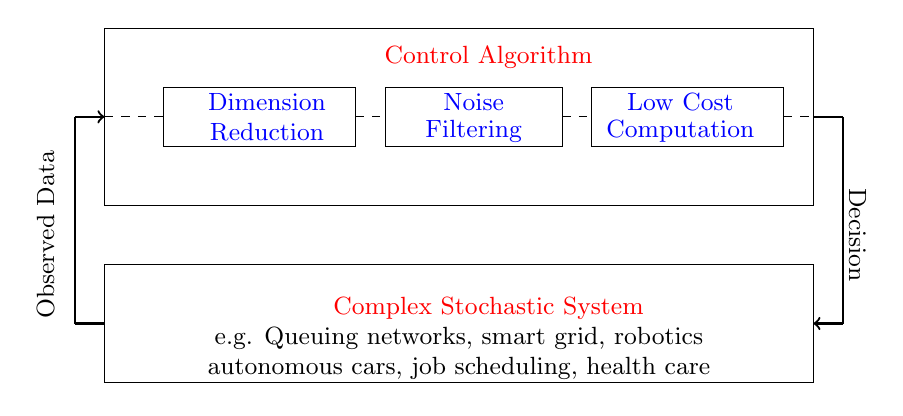
\begin{tikzpicture}[scale=0.75,font=\small,axis/.style={very thick, ->}]
%\draw [black](-2.25,-1) rectangle (2.25,2);
%\node[blue] at(0,1.75) {Modelling};
%\node[blue] at(-1.5,-1.5) {MDP};
%\node[blue] at(-1.5,-1.8) {\&};
%\node[blue] at(-1.5,-2.1) {SMPL};
%\draw[thick,->](-1.5,-1.4)--(-1.5,-0.75);






%\node[blue] at(8,-1.5) {ADP,RL,SPSA};
%\node[blue] at(8,-1.8) {\&};
%\node[blue] at(8,-2.1) {RL};

%\draw[thick,->](8,-1.4)--(8,0.1);
\node[red] at(4.5,4.5) {Control Algorithm};
\draw[black](-2,5) rectangle (10,2);


\draw [black](-1,3) rectangle (2.25,4);
\node[blue] at(.75,3.75) {Dimension};
\node[blue] at(.75,3.25) {Reduction};

\draw [black](5.75,3) rectangle (2.75,4);
\node[blue] at(4.25,3.75) {Noise};
\node[blue] at(4.25,3.25) {Filtering};

\draw [black](6.25,3) rectangle (9.5,4);
\node[blue] at(7.75,3.75) {Low Cost};
\node[blue] at(7.75,3.25) {Computation};

\node[red] at(4.5,0.25) {Complex Stochastic System};
\node[black] at(4,-0.25) {e.g. Queuing networks, smart grid, robotics};
\node[black] at(4,-0.75) {autonomous cars, job scheduling, health care};
\draw[black](-2,1) rectangle (10,-1);

\draw[thick,->](-2.5,3.5)--(-2,3.5);
\draw[thick,-](-2.5,3.5)--(-2.5,0);
\draw[thick,-](-2.5,0)--(-2,0);

\draw[dashed,-](-2,3.5)--(-1,3.5);
\draw[dashed,-](2.25,3.5)--(2.75,3.5);
\draw[dashed,-](5.75,3.5)--(6.25,3.5);
\draw[dashed,-](9.5,3.5)--(10,3.5);

\draw[thick,-](10,3.5)--(10.5,3.5);
\draw[thick,-](10.5,3.5)--(10.5,0);
\draw[thick,->](10.5,0)--(10,0);


\node[rotate=90] at(-3,1.5) {Observed Data};
\node[rotate=270] at(10.75,1.5) {Decision};

\end{tikzpicture}

\end{minipage}
\begin{minipage}[b]{0.5\textwidth}
\centering
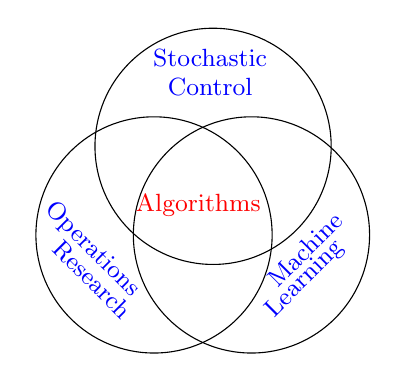
\begin{tikzpicture}[scale=0.75,font=\small,axis/.style={very thick, ->}]
\draw [] (0.9,0.5) circle (2);
\draw [] (-0.75,0.5) circle (2);
\draw [] (.25,2) circle (2);
%\draw [] (-0.5,0.5) circle (2);
%\draw [] (0.5,-0.5) circle (2);
%\draw [] (-0.5,-0.5) circle (2);

\node[red] at(0,1){Algorithms};
%\node[red] at(0,0.5) {Control};
\node[blue,rotate=45] at(1.8,.25){Machine};
\node[blue,rotate=45] at(1.8,-0.25){Learning};

\node[blue,rotate=-45] at(-1.8,.25){Operations};
\node[blue,rotate=-45] at(-1.8,-0.25){Research};

\node[blue] at(0.2,3.5){Stochastic};
\node[blue] at(0.2,3){Control};
\end{tikzpicture}

\end{minipage}


\label{plan}
\captionsetup{font=footnotesize}
\captionof{figure}{On the left is a schematic of a data-driven control algorithm; the observed data is mapped to a decision rule. The challenge is to design control algorithms that are data efficient, computationally cheap and scalable. The right diagram shows the overlap between three areas. Stochastic control has been used to address problems in operations research in the past. A recent trend has been to used machine learning techniques to build data-driven control algorithms.}
\end{figure}

\textbf{Control Algorithms (need and specification):}  As many applications are added by the day, and with the growing complexity, it is imperative to deploy algorithms to compute the decision rules (henceforth to be called as \emph{policies}), an otherwise impossible task for solely analytical methods or heuristics. The schematic of a control algorithm is given in \Cref{plan}, where the algorithm takes observations from the complex stochastic system as input and 
maps it to a policy.  A natural question will then: what is desirable from such a control algorithm? what are the specifications? The following presents a non-exhaustive list.
\begin{itemize}%[leftmargin=*]
\item Scalability: The number of configurations of the system grows exponentially in the number of dimensions.  It is desirable that the algorithms are computationally cheap, and are tractable. %For instance, consider a single traffic junction with $4$ lanes, and each lane with $3$ (low, medium, high) levels of traffic. The problem is completely specified by the $4$-dimensional quantity indicating the levels at the various lanes. However, the size of the state space is $3^4\approx 10^2$. The number of states in a big city with multiple junctions is exponentially large (say $\approx 10^{200}$ for $100$ junctions). Thus it is desirable for the computational costs to grow only as a function of the state variables and not the size of the state space.
 \item Data-Driven: In most scenarios, the underlying model parameters are not known and it becomes important for the algorithms to be solely data-driven. A closely related aspect is that of data efficiency, wherein the algorithms are expected to use all the available information in the given data samples.
\item Performance Guarantee: The algorithms need to be stable, i.e., should produce convergent policies. Further, it is desirable that the computed policy is near-optimal.
\end{itemize}

\textbf{Algorithm Design (tools and techniques):} The schematic (\Cref{plan}) shows the overall template of a control algorithm that is likely to meet the specifications of incurring low computational cost and of being data driven. 
%Markov decision processes (MDPs) is a useful mathematical framework to formulate many stochastic control problems, and forms the basis for design and analysis of a wide family of control algorithms. 
While specific details of the algorithms could vary, all of them can be said to combine three keys components (not in any specific order) namely data assimilation, dimension reduction and low-cost computation. Markov decision processes (MDPs) is a useful tool to formulate stochastic control problems, and the Markovian nature gives rise to the idea of dynamic programming (DP) which forms the back bone of the computational procedure in most of such control algorithms. Ideas of related to dimensionality reduction and noise filtering come from theory of approximate dynamic programming and stochastic approximation respectively. Recent times have also seen the growth of a class of stochastic control algorithms called reinforcement learning (RL) algorithm which combine ideas from a variety of fields such as Markov decision processes (MDPs), approximate dynamic programming (to deal with dimensionality reduction) stochastic approximation  (SA) (to deal with noisy data), and machine learning (to learn from sample trajectories). RL algorithms have been extremely successful in a variety of applications such as queuing networks, autonomous game play and robotics.
%The algorithms are in general sample trajectory versions of approximate dynamic programming that combine ideas of dimensionality reduction and dynamic programming, are model based and computationally cheap. Reinforcement learning algorithms are data-driven algorithms and in most cases are sample trajectory versions of ADP algorithms. RL algorithms are data-driven, and computationally cheap, and have been found to be successful in a variety of applications. Theoretical convergence of RL algorithms follow from stochastic approximation theory. 

\section{Past Work}\label{past}
In the previous section, we saw some specifications and design techniques for control algorithms to address the question of computing near-optimal policies. Naturally, the following question of interest: are computationally cheap data-driven methods stable? do they give useful policies? how fast do they estimate? I was fortunate to contribute towards the answering these questions during the past years.

\textbf{ADP in $\minp$ basis:} A widely used dimensionality reduction technique is linear function approximation, wherein, the value function is approximated by the linear combination of set of chosen basis functions. By choosing fewer basis functions (in comparison to the size of the state space), the ADP algorithm is dimension free.
One of the important issues with such ADP is that even the most fundamental methods such as approximate value iteration/policy iteration (AVI/API) don't have convergence guarantees, i.e., the computed sequence of policies can diverge. In our work \cite{cdc}, we showed that if the basis is chosen to be $\minp$ linear (also known as tropical-linearity), then the ADP methods will be convergent and the performance of the computed policy depends on the function approximation.  

\textbf{Constraint reduction in approximate linear program:} The approximate linear program (ALP) is an ADP method that has performance guarantees \cite{alp} for the computed policy and is guaranteed to converge (unlike other AVI/API). A limitation of the ALP is the intractably large number of constraints. In our work \cite{alp-aaai,alp-ieee}, we provided theoretical guarantees for constraint reduction in ALP. Our arguments are based on geometry of the linear programs as opposed to previous works based on counting (VC-dimension) based arguments. We showed that the performance of ALP can be guaranteed by choosing the constraints corresponding to a \emph{conic-cover} of the given basis functions.

\textbf{Stability:} We derived conditions that imply stability and boundedness of multi-timescale stochastic approximation (SA) algorithms. Our work significantly extended the prior work on stability of single timescale SA algorithms \cite{borkar-meyn}, and provided a blanket result \cite{automatica}, that covers a widely used class of reinforcement learning algorithms called actor-critic methods. 

\textbf{Finite-Time Performance:} Temporal difference (TD) class of learning algorithms have been widely used to learn value functions of a given policy. Such value function learning is a sub-loop in many important RL algorithms (such as actor-critic methods). Many of the important TD algorithms are also linear stochastic (LSA) approximation methods. The choice of the stepsize or learning rate is critical for the performance of LSA algorithms. In our work \cite{aistats}, we studied LSA with constant stepsize and iterative averaging, and showed that TD algorithms can be deployed with a universal constant stepsize, and achieve a problem instance dependent $O(1/t)$ rate for the convergence of mean-squared estimation error. Our work eliminates stepsize tuning in a host of TD algorithms.

I was also fortunate to work of some interesting control problems in crowd-sourcing and Hadoop. In our work \cite{hcomp}, we showed that learnt optimal pricing policies achieve better completion times for the tasks posted onto a crowd-sourcing platform. In our work \cite{hadoop}, we proposed a noisy gradient algorithm to tune the parameters in Hadoop framework; our approach achieved $25\%$ to $60\%$ improvement in performance over the default parameter setting.

%\textbf{Crowd-sourcing:} is a new paradigm wherein tasks that are difficult for computers but easy for humans are solved in a decentralized manner. Here, such tasks are posted on to crowd-sourcing platforms (such as Amazon Mechanical Turk, Crowdflower), to be picked by crowd-workers, who can finish such tasks in their free time. The price offered to the workers for completing is a critical factor that determines the time taken to complete the tasks.  In our work \cite{hcomp}, we considered the problem of optimal pricing of crowd-sourced tasks, with an aim to achieve timely completion. We collected real-time data from CrowdFlower, learnt the underlying MDP, solved for the optimal pricing policy and deployed the pricing policy in real-time, which achieved significant improvement over uncontrolled policies.

%\textbf{Hadoop:} The performance critically depends on tuning parameters.

\section{Future Work}\label{future}
 I strongly believe that new practical application problems give rise to new design specifications and algorithmic ideas. Thus, I strive to strike a healthy balance between theoretical questions as well as practical problems in stochastic control.
 
 \textbf{Constrained and Risk-Sensitive Control:} Several applications need policies to satisfy one or more constraints. For example, in energy harvesting sensor networks, each sensor is constrained by the amount of energy it can expend at any given time, or an autonomous driving system has speed limitations while navigation, or a stock investment policy cannot fluctuate the portfolios in a non-smooth manner. Another aspect is that of risk-sensitivity, i.e., the policies are not supposed to visit certain \emph{dangerous} states. For example, while controlling a autonomous helicopter, there could be states that lead to instability and eventually cause the overall system to crash. Thus, developing reinforcement learning algorithms for risk-sensitive and constrained control problems is an interesting research direction with a variety of applications.
 
 \textbf{Exploration vs Exploitation:} An important stochastic control problem is that of efficient data assimilation, i.e., based on prior data we need a policy that learns about the environment in an optimal way. An example application is health care, wherein, it is important to gather maximum patient information while making minimal possible tests. Also, in many applications the feedback might be complex, i.e., we can obtain the rewards only for a group of actions (by several decentralized control units), or the feedback is delayed. Typically, these problems are posed as multi-armed bandit problems, while the independent arms case and the linear MAB problems have been well understood in literature, newer applications typically require significant modification of the basic MAB algorithms. In particular, multi-agent systems such as sensor networks, or robots, decentralized MAB algorithms are required for effective co-ordination via optimal communication.
 
 \textbf{Classical vs Learning based Control:} Classical control as well as learning based algorithms have the same objective, i.e., to produce a decision rules. However, the approaches in both the areas are quite different. Classical control is mostly model-based and learning based algorithms do not worry about the model, but instead are geared towards design of solely data-driven controllers. Specifically, several learning control algorithms have deep neural networks (DNNs) as their integral part, and several questions are still open: why do DNNs generalize? when are DNNs trainable? when do DNNs produce reliable policies. An interesting research direction is to use tools from control theory to answer some of the questions. For instance, several training algorithms for DNNs such as Nestrov's accelerated gradient have be interpreted as dynamical systems, and tools from robust control theory have been used for principled design of these algorithms. As we move forward to newer applications, developing and analysis hybrid controllers based on classical as well as learning techniques is of interest.
 
 \textbf{Vision and Control:} A common thread connecting some of the recent success of learning based control such as Atari, AlphaGo, autonomous driving, is that the input is a vision signal.  A general view is that vision signals are rich in representing the underlying environment and by learning the inherent symmetries in the vision input can help in efficient control. This leads to an interesting question in the other direction: can control policies also dictate attention towards particular parts in the field of view to gain useful information? To answer these questions, it is important to pose a combined vision and control problem to design newer algorithms.
 
\section{Conclusion}
This document outlines some of my past and future research directions n the area of algorithms for stochastic control. These plans and directions are in various levels of concreteness; some of them require significant extension of existing theory, other require newer mathematical formulations. Most of these problems have well founded application areas as well. I also believe that these questions are inherently flexible to cater the interests of most students. The list of directions are not exhaustive and I will be constantly strive to add newer directions with the progress of time.
\bibliographystyle{plain}
\bibliography{refnew}

\end{document}
